\subsection{Modelo}

Recall that the main objective of access to data is to obtain knowledge. You have to have in
Account that the data by themselves, do not have any value, since they lack sense, once integrated in a context,
will provide us with information, and by processing and analyzing this information, we will obtain the knowledge. \\
    
\begin{figure}[ht]
    \centering 
    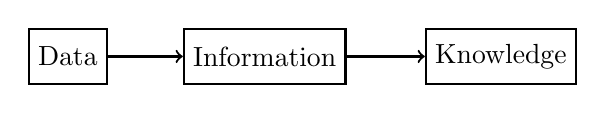
\begin{tikzpicture}[thick]
        \node[draw,rectangle,minimum size=20] (a) {Data};
         \node[draw,rectangle,minimum size=20,right of= a, node distance=2.5cm] (b) {Information};
         \node[draw,rectangle,minimum size=20,right of=b, node distance=3cm] (c) {Knowledge};
         \draw[->] (a) to (b);
        \draw[->] (b) to (c);
     
      \end{tikzpicture}
      \caption{Diagrama. De datos a conocimiento}
    \end{figure}
 
    In order to obtain this knowledge of the data, it is necessary that the user correctly interprets the data, not
    simply that they mean the values and the units, but they represent. For the
    that the user must have knowledge in the matter or perform a research task, which allows
    understand the data extracted.
    
    In order to build a system that makes data accessible, it is essential to design a model to specify the
    information that you want to obtain. The design of a system will allow that, based on given values, provide some results.
    For this it will be necessary to have a solid knowledge of the data set that is needed, the values,
    their units and how they relate to each other.


\subsubsection{How to solve it} 
Study the objective sought and resort to the help of experts if necessary to acquire the necessary knowledge
on the subject. Design a model that provides the information we are looking for.

\subsubsection{How we solve it. Aire Guru} 
Air Guru aims to increase the awareness of the level of pollution that surrounds us, for it uses a measure called
the air quality index (AQI), specifically the European air quality index (EAQI).


\newpage
\begin{figure}[ht]
    \centering
    \includegraphics[width=10cm]{mapAireGuru}
    \caption{Aire Guru. Landing page. Top section}
\end{figure}

It shows the AQI in the whole city of Malaga by zones, both the general and the AQI of each of the agents
contaminants in a more disaggregated form from September 2018 to the present. It also shows the evolution
of these for days, months and years.
It is capable of making a discrimination of the set of most relevant polluting agents by medical conditions.
As an innovative feature, it shows the exhibition at a particular level by hour, day, month, year and the function of
informative glossary.

\elsparagraph{Evaluation}  

\begin{itemize}
\done The information is focused on an objective, informing the user of the level of pollution that surrounds it in real time
and in the past
\done The information follows a logical thread. Storytelling
\done The web offers information, not just data
\end{itemize}

\newpage